% !TEX root = writing_version.tex

\label{chp:data_analysis}
%\section{Diffusion of the lqiuid}
%\label{sec:diffusion_liquid}
%This contain analysis of diffusion in the liquid to prove the simulations accuray
\section{Parameter choice of the simulated system}
\label{sec:system_choice}
As an integral part of this work large scale simulations have been executed on the NEMO High performance computation (HPC) cluster. The input parameters of the simulated systems are given in \autoref{tab:system_1m}.

\begin{table}[ht]
\centering
\begin{tabular}{c|c}
Parameter & Value \\ \hline
N & 1048576 \\
eq\_steps/particle & 1000 \\
pr\_steps/particle & 20000  ... 60000 \\
$\eta_i$ & 45.0 \% \\
$\eta_f$ & 53.1\% ... 53.4 \% \\
\end{tabular}
\caption[Simulation parameters of data production systems]{Input parameters of large scale simulations on the NEMO HPC cluster. The varying steps during production come by the fact, that 20000 steps were estimated to be calculated within 3 days leaving 1 day of buffer to the hard wall time limit of 4 days. Due to the increasing calculation cost of the q6q6 cluster routines for large clusters the wall time limit was still breached and without proper reset steps the datasets could not be restarted without large calculation overhead as all lost data has to be replaced, and the broken reset steps within the files would have to be removed prior to further simulations. Therefore the last proper version of the files were used resulting in varying simulation lengths but with usually a nucleation event in case of early breakdown.}
\label{tab:system_1m}
\end{table}

The simulations consist of four series at volume fractions of $\eta = 0.531,\;0.532,\;0.533,\;0.534$, where each series again consists of 500 trajectories. Therefore at each volume fraction a total number of about half a billion particles have been simulated in the metastable fluid.\\

The volume fractions have been chosen too probe nucleation to the lowest possible limit. As single nucleations have been observed down to volume fractions of $\eta=53.2\%$, the lowest volume fraction was set to just below this value, as the large statistic of 500 trajectories was expected to still yield enough nucleation events to measure the nucleation rate.\\

The size of the systems was chosen comparably large with about 1 million particles. These large systems intuitively seem to be in conflict with the long induction times, even though using CNT as a guideline it can be shown that the computational effort for simulating nucleation events does not significantly increase with increasing system size. The calculation time per unit of simulation time is proportional to N, it is at a given volume fraction also proportional to the volume V:
\begin{align}
\label{eqn:system_size}
\frac{T_{CPU}}{\delta t_{Sim}} \propto N \propto V 
\end{align}

Further we expect the nucleation time in terms of the system time $\langle \tau_{Nucleation} \rangle$ to be proportional to the inverse of the system volume if assuming a nucleation rate density independent of time:
\begin{align}
\langle \tau_{Nucleation} \rangle \propto \frac{1}{V}
\end{align}

As the required CPU time for a nulcleation event is simply proportional to the product of $\langle \tau_{Nucleation} \rangle$ and the calculation time per unit of system time we can conclude:

\begin{align}
\langle T_{CPU} \rangle \propto  \frac{T_{CPU}}{\delta t_{Sim}}  \cdot \langle \tau_{Nucleation} \rangle \propto \frac{V}{V} = \text{const.}
\end{align}

Thus the size of the system is only relevant to be chosen smaller if ordering processes are important for the system resulting in an induction time that is independent of the system size. This might be the case for polydisperse systems, but in the monodisperse case the above reasoning was found to hold true.\\
An other objective that has to be considered is that less configuration snapshots of the system can be stored, as these requrie a lot of space. If one is interested in quantites like $g(r)$ this is not a problem as the necessary statistics can be either derived from a large set of small snapshot or from a small set of large snapshots, but for example resolving and storing the dynamcs of a configuration for a growing cluster would require using smaller system sizes as files easily grow to many GB's in size. 

\section{Long time diffusion time scale}
\label{sec:diffusion_metastable_liquid}
Diffusion or more precisely self-diffusion, characterizes the movement of the single particles within the system. The diffusive behavior for many system can be subdivided into different regimes with different physical meaning.\\ 

For the ballistic hard sphere system we have an extremely short period in which most particles are freely moving without constraint, the ballistic regime. This could be resolved in the simulation by taking measurements at extreme rates, like after every event, but is not as the result could if desired also be determined by measuring the velocity distribution.\\ 

The short time diffusion usually seen in many systems is not seen in the ballistic hard sphere system. To understand this we can look at the physical interpretation of the short time diffusion. While it does not describe the movement of particles between different liquid cages, it only describes the Brownian motion of particles in the suspension within their momentary liquid cage. As the simulated system does not contain any suspension there is no short time diffusion.\\

The long time diffusion on the other hand describes the movement of single particles in the simulated systems on long time scales. The interpretation of the long time diffusion is that particles are able to change their momentary cage by collisions and thus can diffuse throughout the whole system until finite size effects stop their further diffusion. If circumventing finite size effects by using unwrapped coordinates the long time movement of the particles is governed by the relation \autoref{eqn:einstein_relation} which was first described by Einstein\cite{Albert1905}.

\begin{align}
\label{eqn:einstein_relation}
D^S_L = \underset{t\rightarrow \infty}{\text{lim}} \frac{\langle (\vec{r}(t) - \vec{r}(0) )^2 \rangle}{2 d t}
\end{align}

With $D^S_L$ the long time self-diffusion constant which will in the following be denoted only by D, $\vec{r}(t)$ the position of a particle at time t, d the number of spatial dimensions of the system and $\langle ... \rangle$ the expectation value of the ensemble.\\

The average is measured in the system by saving an reference position of all particles at one point, and further carrying a set of unwrapped positions through out the simulation. The average of all particles difference in their reference position with their unwrapped position is used as a measurement of the ensemble average. Especially for large system of 1 million particles, this quantity has only very small fluctuations as can be seen in \autoref{fig:diffusion_comparison}.


\begin{figure}[ht]
\begin{center}
\subfloat[Histograms of the slopes for the linear regressions to the mean squared displacements. The histograms are for $\eta=0.531,\;0.532,\;0.533,\;0.534$.]{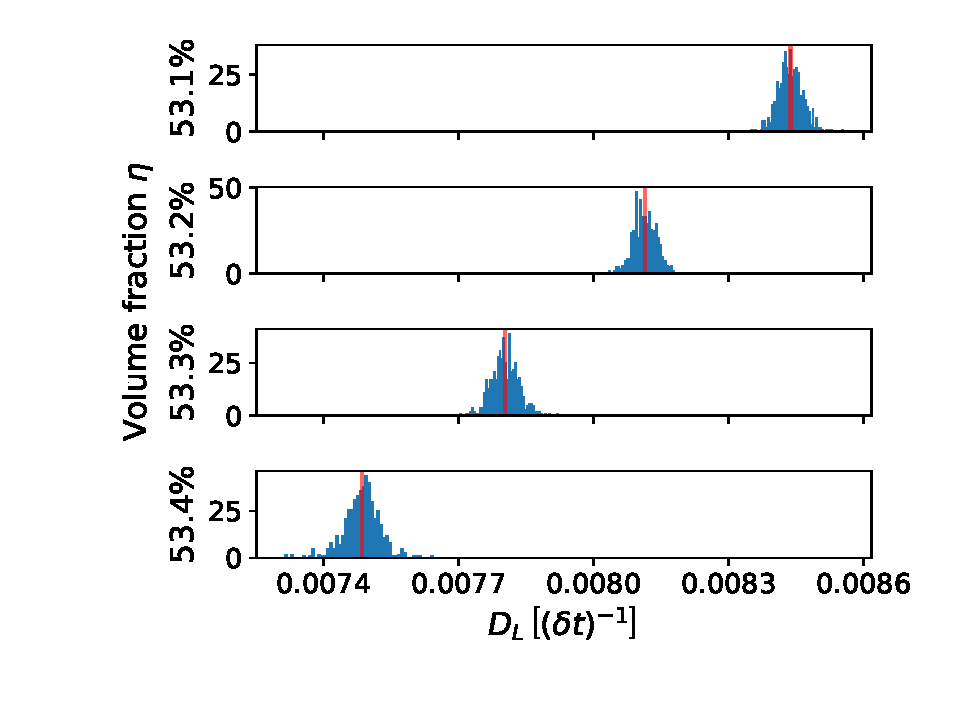
\includegraphics[width = 0.45 \textwidth]{diffusion_histogram_comparison.pdf}} \hspace{0.5cm}
\subfloat[Mean of the histograms with the uncertainty on the mean given by $\sigma_{\langle D \rangle} = \sigma_D/\sqrt{n}$ with n being the number of measurements included in the average.]{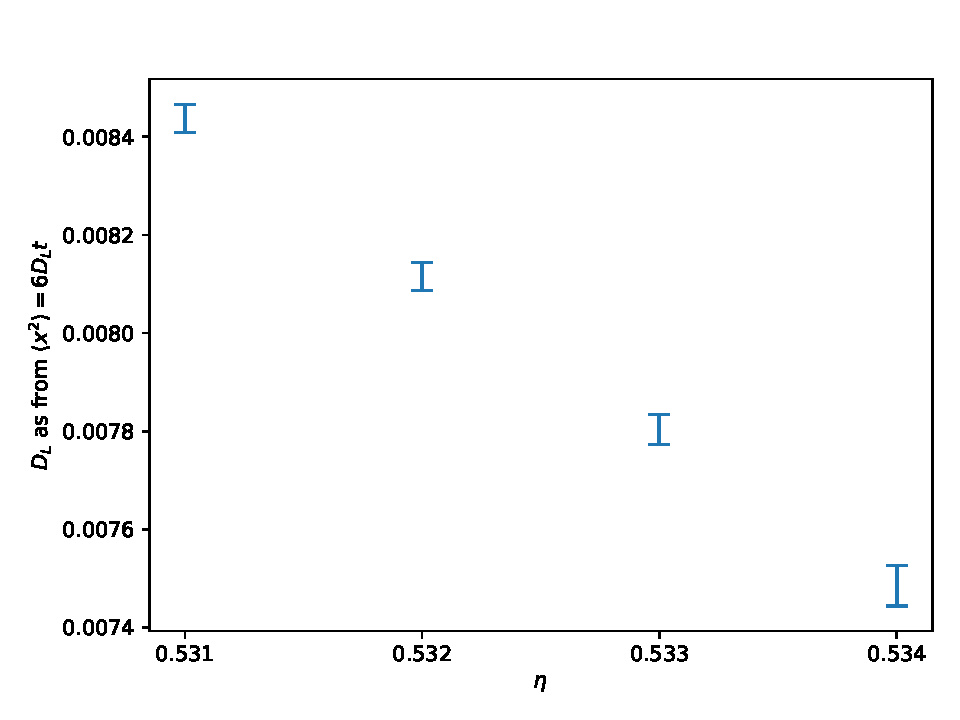
\includegraphics[width = 0.45 \textwidth]{diffusion_comparison.pdf}}  
\caption[Long time self-diffusion constant measurements from production data]{Comparison of long time self-diffusion constants at different volume fractions as histograms and their means with uncertainty.}
\label{fig:diffusion_comparison}
\end{center}
\end{figure}

The diffusion coefficients are important to know for comparison between different systems. This importance is based on the idea that the fundamental mechanisms for nucleation and cluster growth do not vary between different hard sphere like systems, but are only scaled by the varying diffusion times. Furthermore there are theoretical predictions for the relationship of short time and long time diffusion, making it possible to compare experiments where the short time diffusion behavior is better accessible with the ballistic simulations where only the long time diffusion constant is measurable.\\


As we see in \autoref{fig:diffusion_comparison} the diffusion constants can be measured with rather good precision with a relative standard deviation of $\sigma_D/D \approx 1\%$. Hence it does not introduce large uncertainties when normalizing time related quantities by the diffusion time $\tau_{D} = D^{-1}$.

\section{Cluster size distribution over time}
\label{sec:pnt}
The cluster size distribution of the system can be used to test the assumption of Markovian dynamics by trying to find a Fokker-Planck equation describing the time evoluation of the distribution. This has been done for the Lennard-Jones system by Kuhnbold et al.\cite{Kuhnbold2019}. Testing the trajectories shown in \autoref{fig_pnt_short} and \autoref{fig_pnt_long} in a similar fashion would yield a good comparison but due to time constraints of this thesis it is not done. We still can illustrate some characteristics of the metastable fluid directly after and long after the quench as it compactly shows some main features of the system.\\ 

The cluster size distributions are the averages over all trajectories at a given volume fraction. While they are normalized by the number of included measurements they have not been normalized by the volume. The maximum cluster size is set to 160 as above this value only nucleating trajectories can be seen. Also a logarithm to the base of 10 is used, and cluster sizes not present at a given time step have been fixed to a value below the minimal signal as the logarithm requires non zero values.\\
The logarithmic representation is used as the mesurements span orders of magnitude and further can be interpreted as a quantity proportional to a free energy under the logarithm. This is justified by assuming that stationary states may fluctuate in a free energy landscape where the probability for a particular state with some energy $\delta E$ follows a Boltzmann distribution $p\propto \exp \left( - \frac{\Delta E}{k_B T} \right)$.\\

\begin{figure}[ht]
\begin{center}
\subfloat[$\eta = 53.1\%$]{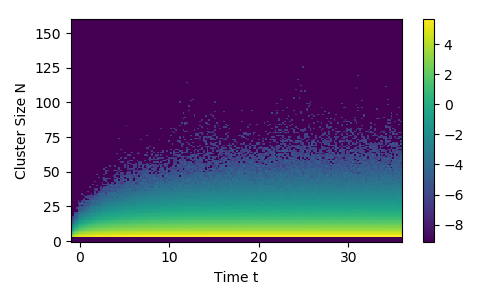
\includegraphics[width = 0.49 \textwidth]{pnt_531_short.png}} \hspace{0.0cm}
\subfloat[$\eta = 53.2\%$]{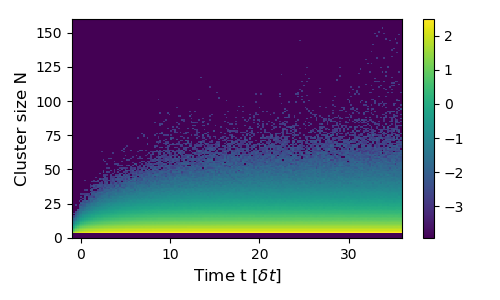
\includegraphics[width = 0.49 \textwidth]{pnt_532_short.png}}\\
\subfloat[$\eta = 53.3\%$]{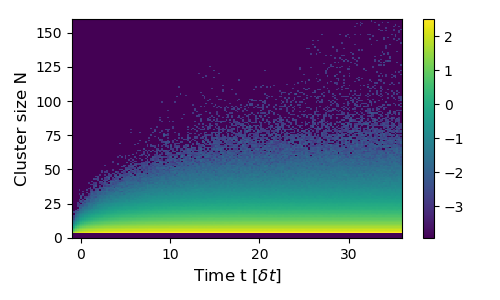
\includegraphics[width = 0.49 \textwidth]{pnt_533_short.png}} \hspace{0.0cm}
\subfloat[$\eta = 53.4\%$]{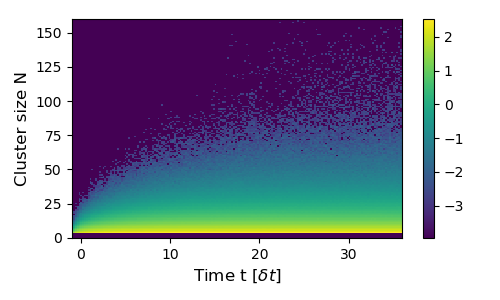
\includegraphics[width = 0.49 \textwidth]{pnt_534_short.png}}
\caption[Cluster size distributions over time after quench]{Cluster distributions at different volume fractions in the initial phase after the quench.}
\label{fig:pnt_short}
\end{center}
\end{figure}

In \autoref{fig:pnt_short} we can see the initial phase after the quench. As the fluid before the quench was at a volume fraction of $\eta=45\%$ only very little local ordering is present directly after the quench. This changes within the first $15 -25 \delta t$ after which the distribution becomes stable, where the interval lenght depends on the volume fraction. As this first time interval shows how long it takes for the system to build up the local ordering in the metastable liquid, and the unstable clusters tend to be larger for higher volume fractions the length of the interval might be explained by the larger number of particles required to find its ordering.\\ 
To further compare the system time with the more intuitive number of collisions each particle had on average we can use that at the given volume fraction we find  $1\delta t \approx \frac{60 steps}{particle}$. When further using a collision probability of $\sim 40 \%$ for each executed event, we find that $1\delta t \approx \frac{25 collisions}{particle}$. As a result we can conclude that it takes a few hundred collisions for each particle to build up the local ordering with unstable clusters.\\

\begin{figure}[ht]
\begin{center}
\subfloat[$\eta = 53.1\%$]{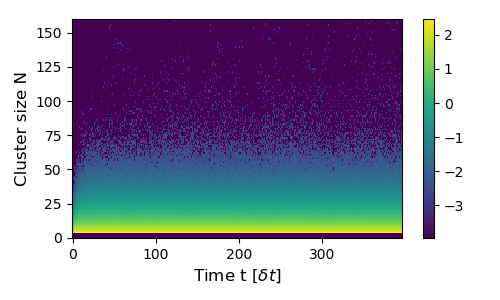
\includegraphics[width = 0.49 \textwidth]{pnt_531_long.png}} \hspace{0.0cm}
\subfloat[$\eta = 53.2\%$]{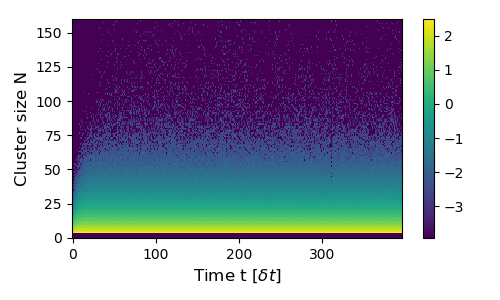
\includegraphics[width = 0.49 \textwidth]{pnt_532_long.png}}\\
\subfloat[$\eta = 53.3\%$]{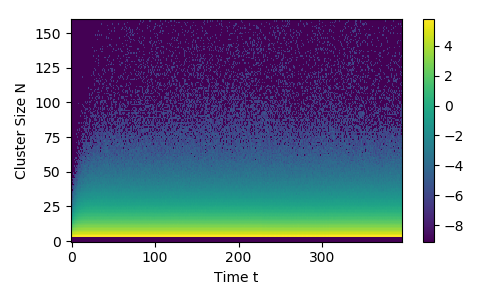
\includegraphics[width = 0.49 \textwidth]{pnt_533_long.png}} \hspace{0.0cm}
\subfloat[$\eta = 53.4\%$]{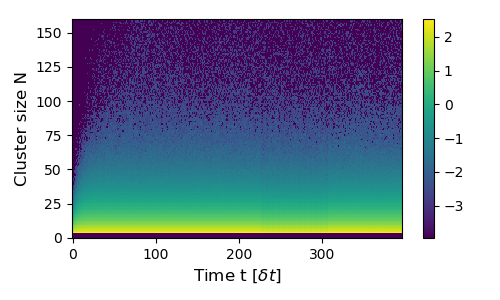
\includegraphics[width = 0.49 \textwidth]{pnt_534_long.png}}
\caption[Cluster size distributions for long waiting times]{Cluster distributions at different volume fractions during the waiting time.}
\label{fig:pnt_long}
\end{center}
\end{figure}

The diagrams in \autoref{fig:pnt_long} show a zoomed out version of the same data depicted already in \autoref{fig:pnt_short}. We see that the distribution that is reached at the end of the initial phase remains stable over prolonged periods of time. Only the nulceation events, which account for most of the probability at largest cluster sizes, indicate that this is not a stable process.

\section{Autocovariance functions of largest cluster in the metastable fluid}
\label{sec:acf}
The autocovariance function (ACF) of the largest cluster contains information about how long a single cluster persists as the largest cluster within the volume, as fluctuations of clusters at different points of the volume are expected to be independent of each other, only the size fluctuation of a distinct cluster should be correlated in time.\\

The autocovariance function is defined by \autoref{eqn:definition_acf}, where $N_{\text{lc}}(t)$ is the number of particles in the largest cluster at time t, $\langle N_{\text{lc}} \rangle_t$ is the corresponding average over time, thus $X(t)$ describes the deviations from the average. The autocovariance function furthermore is normalized by ${ \langle X^2  \rangle }$, the variance of the data, such that $ACF(\tau=0) = 1 $.

\begin{align}
\label{eqn:definition_acf} 
ACF(\tau)=\frac{ \langle  X(\tau)-X(0) \! \: \rangle } { \langle X^2  \rangle }\\  
\text{with } X(t)=N_{\text{lc}}(t)- \langle N_{\text{lc}} \rangle_t 
\end{align}

The ACF is calculated from the largest cluster measurement for each trajectory. Because soon as a nucleation event occurs the largest cluster will surely be correlated to its former size, only those parts of the measurements that did not involve strong cluster growth are used. Therefore the ACF shown in \autoref{fig:acf} show the correlations of the largest cluster in the metastable fluid.\\

\begin{figure}[ht]
\begin{center}
\subfloat[$\eta = 0.531$]{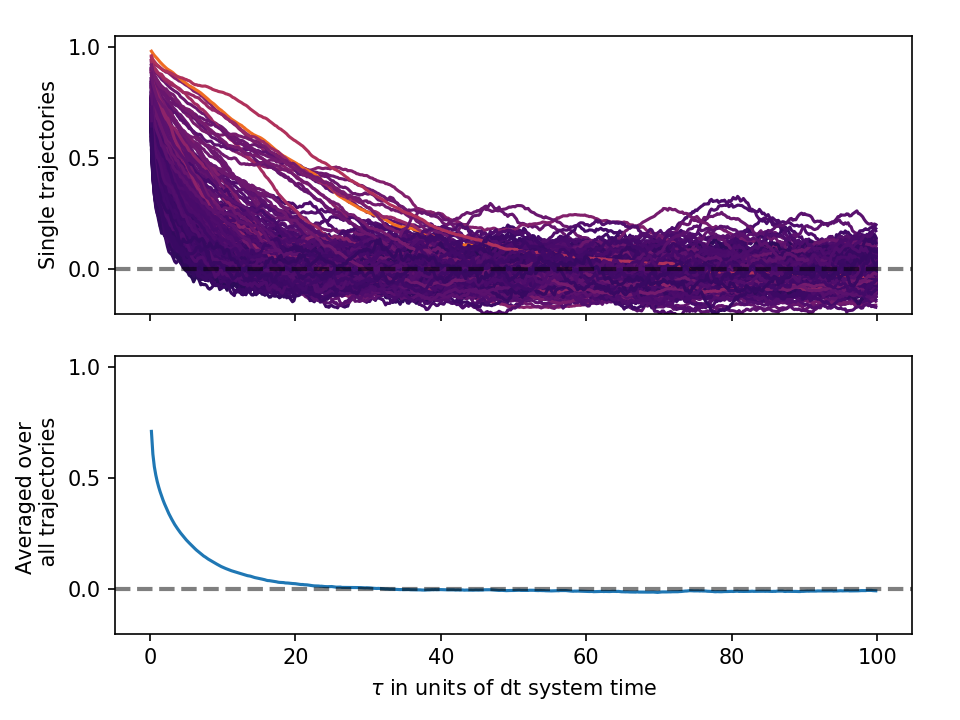
\includegraphics[width = 0.4 \textwidth]{acf_lc_531.png}} \hspace{0.5cm}
\subfloat[$\eta = 0.532$]{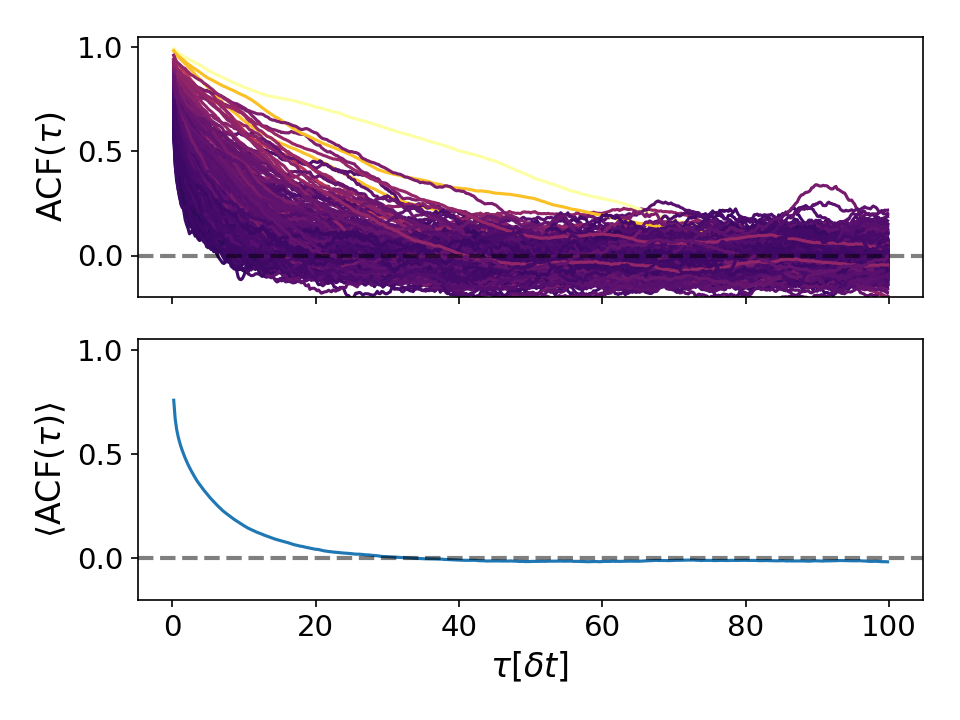
\includegraphics[width = 0.4 \textwidth]{acf_lc_532.png}} \\
\subfloat[$\eta = 0.533$]{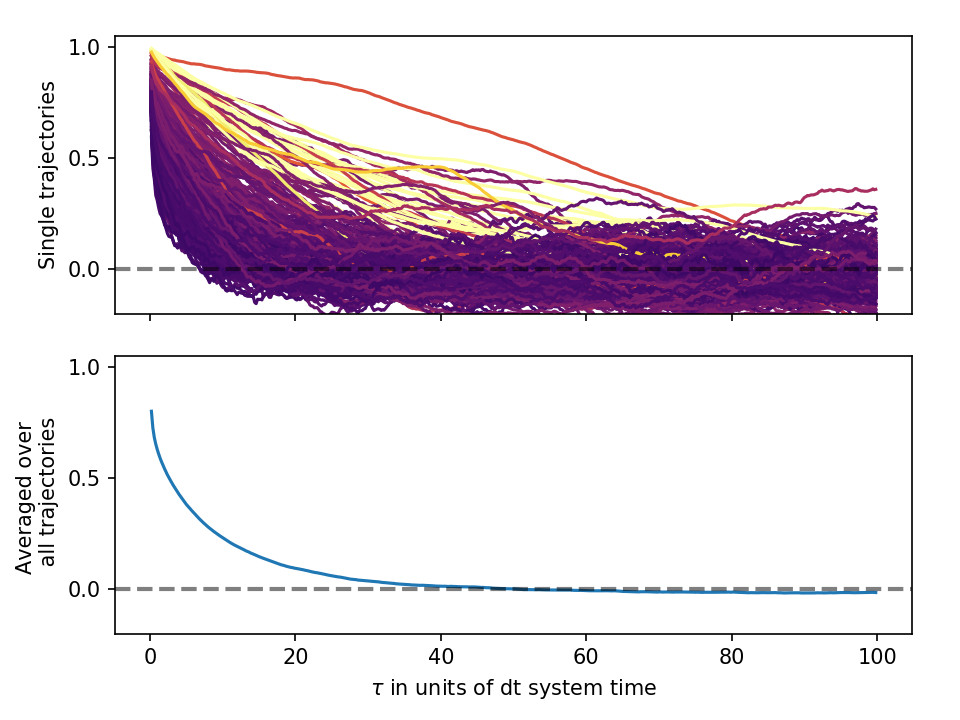
\includegraphics[width = 0.4 \textwidth]{acf_lc_533.png}} \hspace{0.5cm}
\subfloat[$\eta = 0.534$]{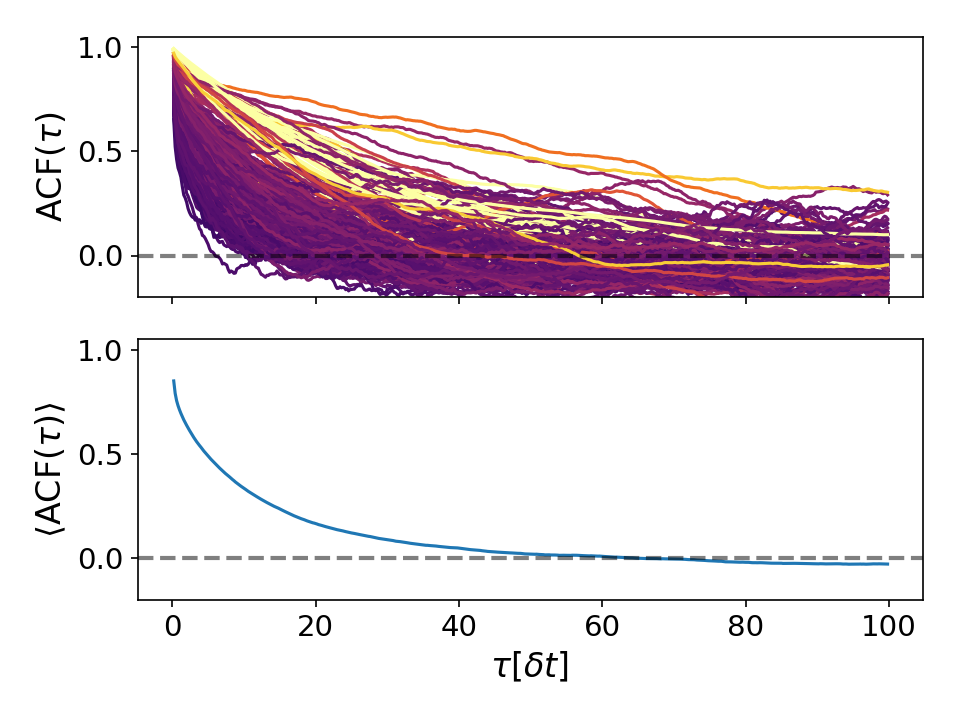
\includegraphics[width = 0.4 \textwidth]{acf_lc_534.png}} \\
\caption[Autocovariance functions of largest cluster in the metastable fluid]{Comparison of autocovariance functions in the metastable fluid. The top of eache diagram depicts all trajectories with coloring indicating the largest cluster size within the used time interval. The lightest color thereby indicates a largest cluster of more than 500 hundred particles which is a nucleation event, but these are rare in the given selection and therefore the data represents the metastable fluid still well. The bottom of each diagram shows the average of the above one with decay times of $ 15 \delta t- 35 \delta t$. }
\label{fig:acf}
\end{center}
\end{figure}

From the autocovariance functions we see that structural fluctuations persist for longer times at higher volume fractions. From the coloring as well as from the cluster distributions we can also conclude that the fluctuations tend to be larger at higher volume fractions and that for $\eta=53.4\%$ a signal from nucleation events might not be completly negligible anymore. Still this behavior was also seen in the cluster size distributions (\autoref{sec:pnt}).\\
Also the time scale on which the ACF decays corresponds closely to the initial ordering time observed for the cluster distribution directly after the quench. And further it also correpsonds to the lifetimes of large clusters found in the single example of the individual cluster tracking algorithm (\autoref{fig:lifetime}). This leads to the conclusion that these three observations all show the same time scale of local ordering processes in the metastable fluid. 

\section{Cluster growth and constant attachement rate}
\label{sec:cluster_growth}
Once the clusters reach a certain size they are expected to grow with new particles being attached to the surface at a constant rate leading to a growth with a proportionality of $N \propto t^3$ as shown in \autoref{eqn:constant_growth} where k is the assumed constant attachment rate, N is the number of particles in a specific cluster, A is the surface of the cluster, R is the radius of the cluster and $\rho_{solid}$ is the bulk density which is for large clusters a good approximation of the cluster density.\\

\begin{align}
\label{eqn:constant_growth}  
\begin{split}
\dot{N} &= k A \\
          & \; \; \, \vrule
  \begin{aligned}[t]
    \quad \text{with}  \quad  N &= \frac{4}{3} \pi R^3 \rho_{solid}\\
    \Leftrightarrow R &= \left( \frac{3 N }{4 \pi \rho_{solid} }\right)^{\frac{1}{3}} \, \text{,} \\
    \quad \text{and}   \quad A &= 4 \pi R^2 \\
    \Leftrightarrow A &= \left(\frac{4 \pi 3^2 }{\rho_{solid}^2} \right)^\frac{1}{3} N^\frac{2}{3} \, \text{,}\\
%    \quad \text{follows} \quad A &\propto N^\frac{2}{3} \\
  \end{aligned}\\
\frac{dN}{dt} &= k \left(\frac{4 \pi 3^2 }{\rho_{solid}^2} \right)^\frac{1}{3}  N^\frac{2}{3}\\
\end{split}
\hspace{1cm}
\begin{split}
%\Rightarrow \frac{dN}{dt} &= c' N^\frac{2}{3}\nonumber\\
%\vspace{0.25cm}\nonumber\\
& \!\!\!\!\!\!\!\!\! \text{From the bottom left side}\\
\Rightarrow& \quad dN \; N^{-\frac{2}{3}} = dt \; k \left(\frac{4 \pi 3^2 }{\rho_{solid}^2} \right)^\frac{1}{3}\\
          & \; \; \, \vrule
  \begin{aligned}[t]
    \quad \text{setting}  \quad  N(t=0) = 0\\
  \end{aligned}\\
\Leftrightarrow& \quad 3 N^{\frac{1}{3}} = k \left(\frac{4 \pi 3^2 }{\rho_{solid}^2} \right)^\frac{1}{3} t\\
\Leftrightarrow&  \quad N^{\frac{1}{3}} = k \left( \frac{4 \pi}{3 \rho_{solid}^2} \right)^\frac{1}{3} t
\end{split}
\end{align}  

As the systems are able to accommodate clusters up to a few hundred thousand particles and usually only one very large cluster is formed during a simulation, the attachment rate can be measured by a linear regression to the third root of the number of particles in the largest cluster over time. This is visualized for the trajectories at $\eta=0.532$ in \autoref{fig:cluster_growth_example}. The volume fraction $\eta=0.532$ is chosen arbitrarily.


\begin{figure}[ht]
\label{fig:cluster_growth_example}
\centering
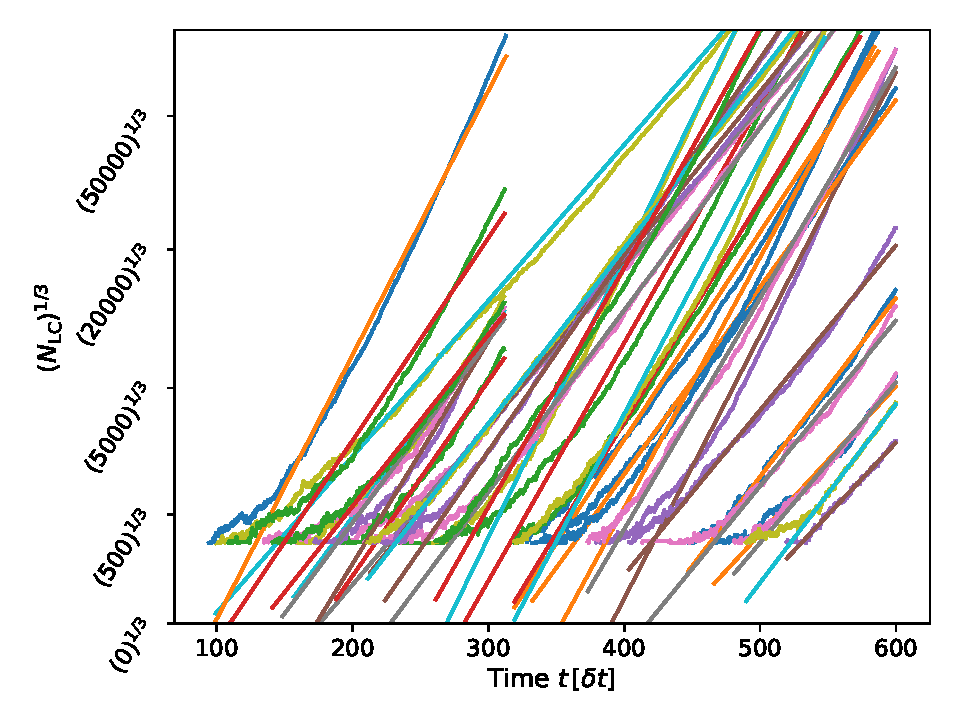
\includegraphics[width=0.7 \linewidth]{cluster_growth_example.pdf}
\caption[Largest cluster trajectories from production data with constant attachment rates]{Trajectories of the third root of the number of particles within the largest cluster of a system over time. Clearly visible is the linear proportionality for which a linear regression is shown together with the data. The cut of some data sets at $t/\delta t \approx 300$ is due to the trespassing of the maximum wall time of the NEMO computational cluster. This means that the simulation of 20000 production steps yields a system time of $T/\delta t \approx 300$. Clusters present already in the first step would become too large in the next simulation interval, leading to a breach of the wall time limit due to the quadratic effort required for the q6q6 cluster finding routine. It can be assumed that clusters forming just around $t/\delta t \approx 300$ might not have been recognized due to this flaw. But as the number of trajectories concerned by this is rather small the impact is not easy to recognize when looking at the induction time distributions in \autoref{fig:induction_distributions}.}
\label{fig:cluster_growth_example}
\end{figure}

Subsequently the slopes of the linear regressions have been collected in histograms shown in \autoref{fig:constant_growth_rates}. As shown in \autoref{eqn:constant_growth} these slopes correspond to constant attachment rates with a dependence on the density within the cluster. As the densities of concern are very close to each other, they only introduce a relative difference of 0.5\% between the rates of lowest and highest volume fractions. For this reason the dependence is neglected for the qualitative comparison.\\ 

\begin{figure}[ht]
\begin{center}
\subfloat[Histograms of the slopes for the linear regressions to the largest clusters during the later stable growth process. The histograms are for $\eta=0.531,\;0.532,\;0.533,\;0.534$.]{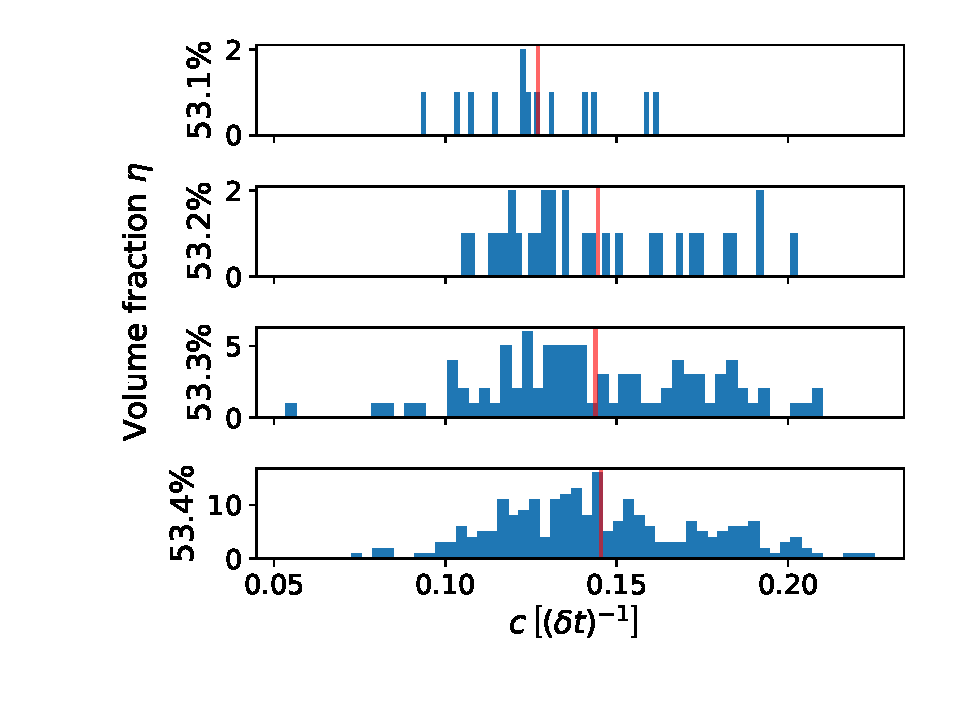
\includegraphics[width = 0.45 \textwidth]{const_growth_rate_histogram_comparison.pdf}} \hspace{0.5cm}
\subfloat[Mean of the histograms with the uncertainty on the mean given by $\sigma_{\langle c \rangle} = \sigma_c/\sqrt{n}$ with n being the number of measurements included in the average.]{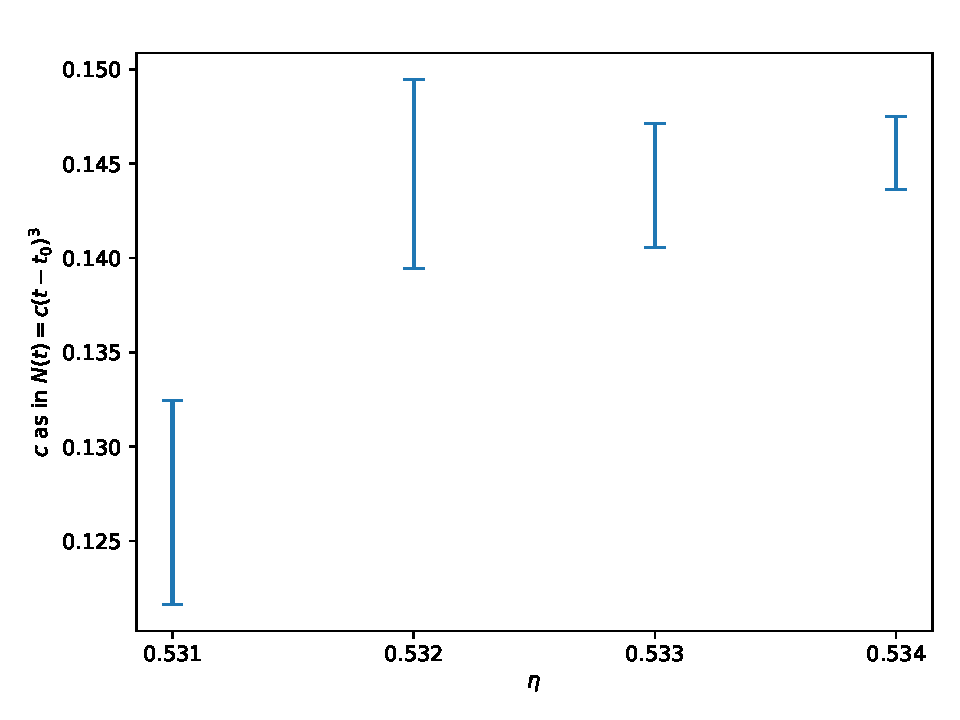
\includegraphics[width = 0.45 \textwidth]{const_growth_rate_comparison.pdf}}  
\caption[Constant attachment rate measurements from production data]{Comparison of growth rates in the constant attachment regime.}
\label{fig:constant_growth_rates}
\end{center}
\end{figure}

What we see from the histograms is that the distribution is rather spread out, but interestingly not significantly depending on the volume fraction. Except for $\eta = 0.531$ we find a smaller growth rate. A possible explanation for this behavior could be that growth by heterogeneous crystallization on the growing cluster surface, leading to a mean higher growth rate for higher volume fractions, is less likely for the lower volume fractions. Either way due to the low statistics at the lowest volume fraction it is also possible that only a statistical fluctuation is seen. From the similarity of the growth rates we can deduce that the attachment of the particles to the cluster is a reaction controlled process. \todo{is there a reasoning for it being a reaction or diffusion controlled process?} \\

As the diffusion constants vary from $D=0.0081|_{\eta = 0.532}$ to $D=0.0075|_{\eta = 0.534}$ they span a difference of about 7.5\%, but does that mean they are either reaction or diffusion controlled, or is their only nothing to see, as the uncertainty on the growth rate is also of the size 5 \% ?

\section{Tensor of gyration evaluation}
\label{sec:tog}
The tensor of gyration is a very useful tool as it describes the second moments of the position distributions. It comprises information about the spatial extent in all three dimensions with commonly  defined quantities being the radius of gyration, asphericity and anisotropy\cite{Theodorou1985}, which are further discussed in the following.\\

The tensor of gyration itself is defined by \autoref{eqn:tensor_of_gyration}.
\begin{align}
\label{eqn:tensor_of_gyration}
&S_{mn}=\frac{1}{N} \sum_{i=1}^{N} r^{(i)}_m r^{(i)}_n\\
\label{eqn:center_of_mass}
&\text{with} \quad \sum_{i=1}^{N} \vec{r}^{(i)} = 0
\end{align}

As described by \autoref{eqn:center_of_mass} the matrix $S_{mn}$ is calculated in the center of mass frame for particles with the same mass. The tensor of gyration can be diagonalized, with the three Eigenvalues $\lambda_1^2$, $\lambda_2^2$ and $\lambda_3^2$. The Cartesian system thereby is chosen such that $\lambda_1^2 \leq \lambda_2^2 \leq \lambda_3^2 $. These Eigenvalues correspond to the spatial extents of the cluster within the Cartesian system in which the tensor of gyration becomes diagonal. From these three Eigenvalues the quantities defined in \autoref{eqn:tog_quantities1} - \ref{eqn:tog_quantities4} are common to characterize clusters of particles.

\begin{align}
\label{eqn:tog_quantities1}
\text{(squared) Radius of gyration:} \quad &R_G^2 = \sum_{i=1}^3 \lambda_i^2\\
\label{eqn:tog_quantities2}
\text{Asphericity:} \quad &b = \lambda_3^2 - \frac{1}{2}(\lambda_1^2+\lambda_2^2)\\
\label{eqn:tog_quantities3}
\text{Acylindricity:} \quad &c = \lambda_2^2 - \lambda_1^2\\
\label{eqn:tog_quantities4}
\text{Relative shape anisotropy:} \quad &\kappa^2 = \frac{b^2 + \frac{3}{4} c^2 }{R_G^4} =  \frac{3}{2} \frac{ \sum_{i=1}^3 \lambda_i^4 }{\left(\sum_{i=j}^3 \lambda_j^2 \right) ^2 } - \frac{1}{2}
\end{align}

For better understanding of the shape descriptors mentioned before, we can have a more detailed look at their interpretation:

\begin{description}
\item[Radius of gyration $R_G$:] \hfill \\ An averaged radius of the structure.
\item[Asphericity b:]\hfill \\ The difference of the largest extent with an average of the two smaller extents. 
\item[Acylindricity c:] \hfill \\ The difference of the smaller extents
\item[Relative shape anisotropy $\kappa^2$:] \hfill \\ A sum of the asphericity and the acylindricity normalized by the radius of gyration to obtain a dimensionless quantity between 0 and 1.
\end{description}

To spot possible correlations between a cluster's shape and it's growth, the three quantities \autoref{eqn:tog_quantities1} - \ref{eqn:tog_quantities4} derived from the tensor of gyration have been plotted against the cluster size and then colored by three scalar quantities characterizing the growth process of each trajectory.\\ 
The first of them is the induction time, as early nucleations might arise from less ordered clusters resulting in a higher asphericity. The second is the constant attachement rate during cluster growth, where similarly one may expect that clusters including more defects may grow slower and also be less spherical. The third quantity is an exponential initial growth rate which is used to characterize how swift the precursor grows into the later crystal, again with the intuition that clusters with a higher asphericitiy may tend to a slower initial growth as theys might be less ordered. For quantifying the initial growth rate, an exponential function has been fitted to the data up to a cluster size of 500 particles.\\
The representation depending on the cluster size is used, to make the different trajectories comparable, as we expect similar behavior for similar cluster sizes. Because the cluster size depending on time becomes almost monotonic for cluster size above a few hundred particles, it mostly is a transformation of the time axis, while the order is only little influenced. Nevertheless it should be kept in mind that this does not constitute a function anymore.\\
Finally the number of particles, as well as the shape descriptors can span many orders of magnitude making logarithmic scales useful.\\

A large overview produced by this procedure is given in \autoref{fig:tog_overview} for the nucleated trajectories at $\eta=0.534$ with the three shape descriptors in the vertical direction and the three scalar coloring schemes in the horizontal direction.\\

A similar approach trying to correlate the three scalar quantities derived for each trajectory have been done, but also did not show any significant pattern.  

\begin{figure}[!h]
\centering
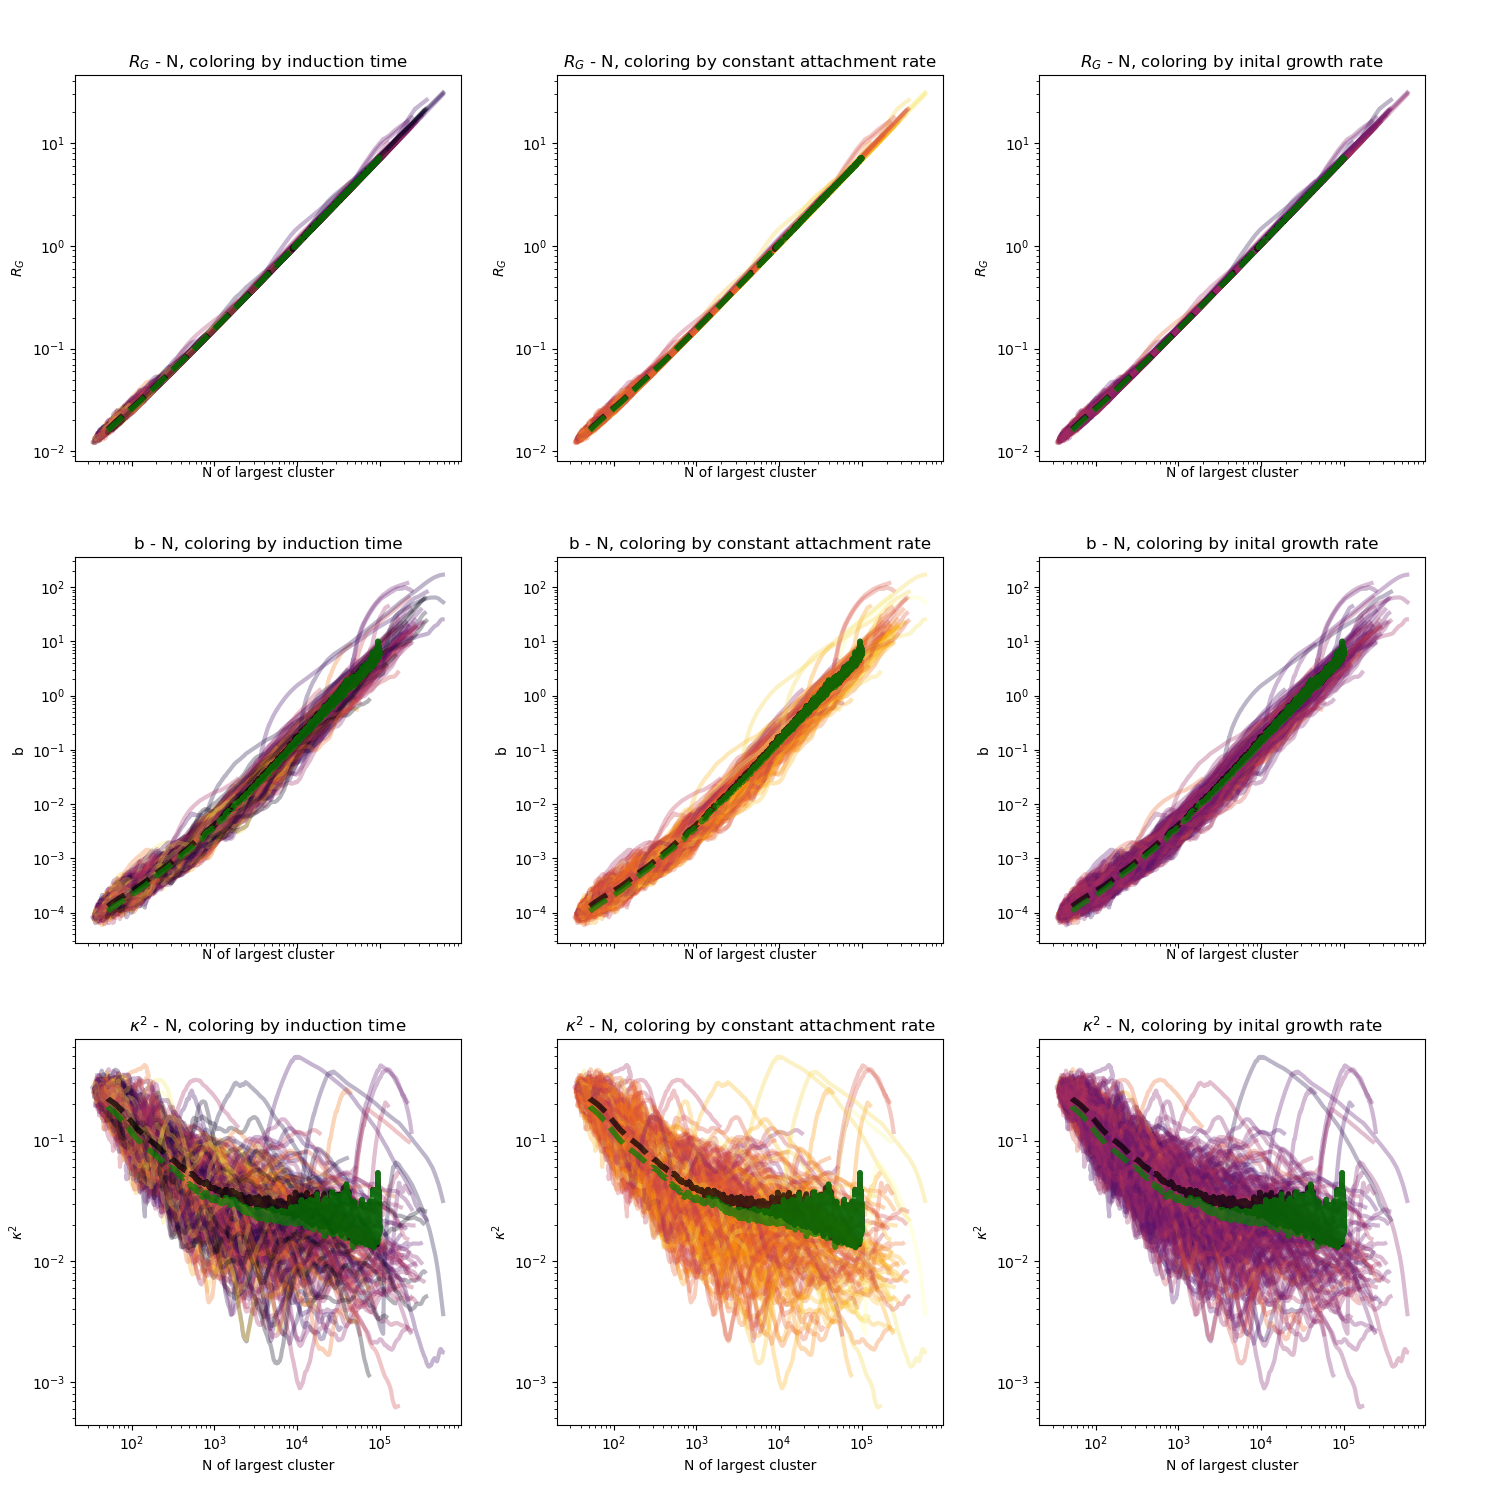
\includegraphics[width=0.8 \linewidth]{Series_534_corrolation.png}
\caption[Tensor of gyration measurements from production data]{Overview of the cluster shape describing quantities: Radius of gyration ($R_G$), asphericity (b) and anisotropy ($\kappa^2$), depending on the size of the cluster. The coloring depicts the scalar quantities induction time, constant attachment rate and initial growth rate. Further a smoothed arithmetic mean and median are calculated and depicted.}
\label{fig:tog_overview}
\end{figure}

From the overview we get no obvious sign that there are any correlations between cluster shape and growth rates or between cluster shape and the induction time. Because of that no deeper analysis is done, but instead we conclude that by this superficial analysis we cannot relate the shape descriptors of the cluster to growth or structural properties.\\

Nevertheless the calculated means give a hint that especially for the anisotropy $\kappa^2$ we can see that up to a size of about 1000 particles the clusters become more spherical while at higher particle numbers this tendency towards a sphere comes to an halt. This could be explained for example by the fact that the clusters always exhibit crystal faces leading to some unavoidable asphericity. An other explanation could be that the attachement rate for one crystal face might be higher than for an other. This also would lead for a single crystal to unspherical growth, but as the clusters arre already rather close to a sphere the attachemnt rate does not seem to vary much between the different crystal faces. Also it has been observed that very large single crystals of a few hundred thousand particles may only form at volume fractions of $\eta = 53.2 \%$. At higher volume fractions on the other side, domains form as it seems that heterogenous nucleation takes place close to the surface of the cluster, leading to a new crystal orientation in the further growth in this spot.\\


\section{Nucleation time dilemma}
\label{sec:nucleation_times}
To calculate induction times or average nucleation times, we will require a definition of when a crystal is called nucleated. This means we have to define from which point a cluster is not merely an unstable fluctuation within the liquid anymore, but instead becomes a stable solid crystalline phase.\\ 
In the literature many concepts are used. For example a cluster can be defined as crystalline soon as its of the critical size, calculated by CNT or by doing a committer analysis. An other possibility often used is to rewind the trajectory in which a clearly stable crystal is found, back to the point where the crystal cluster's size more or less vanishes. A further approach is to fit the growth during later times and extrapolate it to the time when the cluster vanishes.\\

All these definitions differ more or less only by a delay $\Delta_{\tau}$ which is a distribution of times holding the information of how long it takes for varying clusters to pass from the first criterion to the next.\\
For example we can take as a first point the time when a cluster, known to crystallize at later times, cannot be differentiated anymore from any other structural fluctuation in the liquid, i.e. when the size of the cluster falls below some threshold given by the size of clusters regularly present in a given volume.\\
The second point we can set by either the critical size of CNT or by some other criterion when we are sure that the cluster has stabilized and will only continue to grow.\\
At the first of these two points, the fluctuation leading to the crystallization occurs but it would not be possible to tell yet if this precursor melts or continues to grow, while at the second point the crystal is stable. For this reason the first might be called a precursor nucleation and the second crystal nucleation. Between these two points we find the time difference to be the time it takes for the precursors to form a stable crystal. This includes also that some precursors might loiter for awhile before forming the stable phase while other pass this gap rather directly.\\

When calculating a mean induction time, the delay $\Delta_{\tau}$ propagates also to the final result and as it is a stochastic distribution also its higher moments are propagated leading to a smaller precision. This after all only means that the induction time depends on the definition of crystallization and they are only roughly comparable.\\ 
In \autoref{fig:induction_distributions} three distributions with varying definitions of the induction time are visualized.

\begin{figure}[!h]
\centering
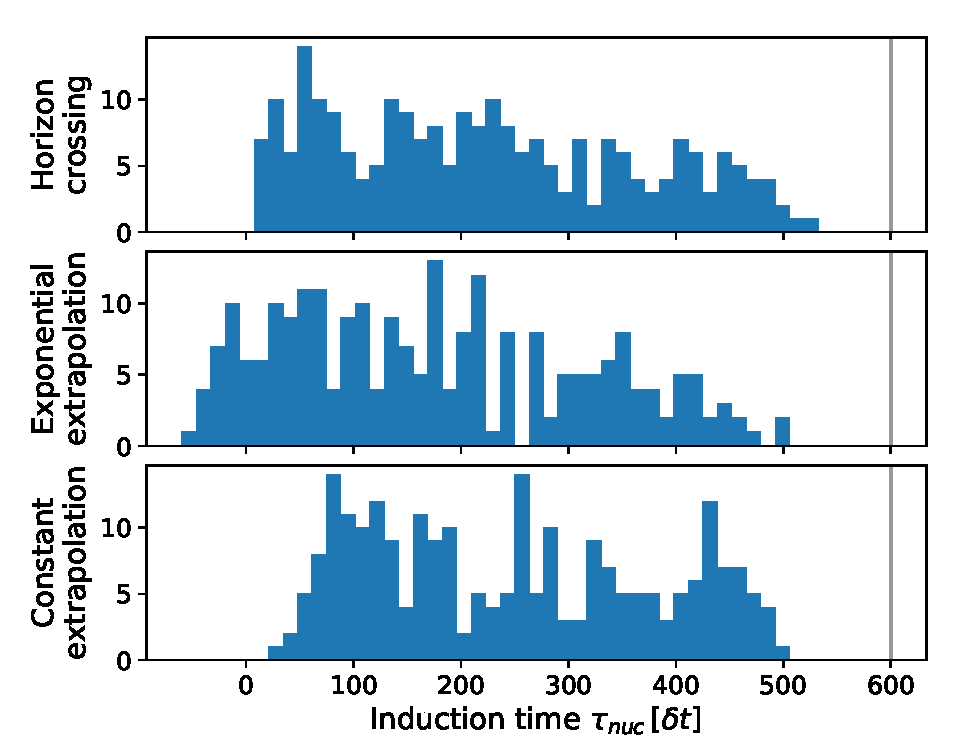
\includegraphics[width=0.6 \linewidth]{varying_induction_time.pdf}
\caption[Comparison of different definitions for the induction time]{Induction time distribution obtained by different definitions. While the two methods using extrapolation seem to have the two effects of smearing the signal as well as shifting them, the method of defining the nucleation as the time when the largest cluster is last below the horizon of fluctuations seems to return the most accurate and precise distribution. The final simulation time is marked by the grey line. As clusters require some time to be clearly recognized as crystals no nucleation events are seen towards the end of the simulation interval. To counteract this we will truncate the distribution in the following analysis such that this does not introduce a bias on the final result.}
\label{fig:induction_distributions}
\end{figure}

The three methods explicitly used here are given by the following:
\begin{description}
\item[Horizon crossing]{The time of nucleation is obtained by following the trajectory of the largest cluster within a system after it clearly nucleated back to the point where it was the last time at the average largest cluster of the metastable fluid without stable clusters. The name horizon crossing refers thereby to the idea that fluctuations of the largest cluster in the metastable fluid are more or less independent fluctuations. This is caused by the fact that the large fluctuations of the system alternate at being the largest one, and therefore the largest fluctuations is not bound locally and the fluctuations becomes independent events. On the other side an extraordinary fluctuation will be seen for a longer period of time as the largest cluster, and thus the corresponding fluctuations are not independent in time. The crossing of the trajectory below this horizon where it cannot be followed any longer is meant by the name.}

\item[Exponential extrapolation]{For this method an exponential growth is fitted to the largest cluster data up to N<500. Extrapolating to smaller times makes it possible to evaluate when the exponential crossed 10 particles, which is then taken as the induction time. The method tends to find negative induction times that are not physical.}

\item[Constant extrapolation]{The name refers to the constant attachment rate found at later times for the cluster growth. It can be extrapolated to earlier times until the cluster has completely vanished i.e N=0. As the constant attachment rate is higher than the initial growth rate this method returns too large induction times.}
\end{description}

As can be seen the horizon crossing method returns a rather smooth distribution that also roughly can be approximated by an exponential decay that is expected for a constant nucleation rate as is shown in \autoref{sec:induction_time_expectation}.\\


\section{Induction time by exponential distribution assumption}
\label{sec:induction_times}
\todo{define nucleation times as well as induction times? It seems like people use them as equivalents.}
Nucleation rates for the meatstable hard sphere fluid have been measured on the experimental as well as on the theoretical side but with a large discrepancy as discussed in \autoref{sec:comparison}. The employed procedures and definitions also vary but not to a point to explain the discrepancy so far. The differences mostly originate from the kind of accessible information and system. While the experimentalists often have access to very large systems but without knowing all positions at all times, theorists mostly have smaller systems in numerical simulations but with the advantage of being able to access all particle positions, and in case of simulations probing the dynamics also all velocities.\\
On the experimental side light scattering and optical methods are mostly employed to measure the structural properties of the probe, comparably on the theoretical side different cluster finding algorithms are used.\\

While experimentalists may define an induction time by the time interval it takes for a quenched system to reach some level of overall crystallinity, theorists have often used simple approaches like the average time to nucleation for a couple of trajectories to measure their induction times\cite{Filion2010a} \todo{cite it here or not?}. This constraints the theorist to wait for all trajectories of an ensemble to show nucleation, what renders it very unsuitable for systems at low volume fractions where the induction time increases steeply.\\

To circumvent this problem we will define the nucleation rate in the following differently without requiring all simulations to nucleate. In fact we can also show that the uncertainty of the induction time obtained from the data is not significantly reduced anymore for measurements longer than the mean induction time.\\

\subsection{CNT expectation of the induction time distribution}
\label{sec:induction_time_expectation}
In \autoref{sec:CNT} we introduced classical nucleation theory and its constant nucleation rate depending on the barrier height in the free energy landscape. Even if there are signs that CNT is not appropriate for describing nucleation process completly, we will use its prediction of a constant nucleation rate as an assumption to define a constant scalar nucleation rate as well, to compare with other literature values.\\

As also mentioned before, in the discussion of the system sizes (\autoref{sec:system_choice}), the induction time of a system depends on the volume under consideration and for this reason the nucleation rate is commonly defined as a nucleation rate density $k$.\\ 
Considering now the simulations we can describe them as a total of $m$ volumes with a size of $V_{box}$.  Further we can define the number of boxes in which a nucleation occurred as $n(t)$ and exclude these from the further simulation.\\

In this case the total nucleation rate $ \dot{n} $ can be written by \autoref{eqn:nuc_rate} from which in the continuous limit of an infinite number of different simulations we can deduce the expected induction rate.

\begin{align}
\label{eqn:nuc_rate}
\dot{n} &= (m - n(t))V_{box}k\\
\Leftrightarrow \frac{\dot{n}}{m} &= (1 - \frac{n(t)}{m})V_{box}k\\
 &  \text{in the limit } m \rightarrow \infty \nonumber\\
\Leftrightarrow \frac{n(t)}{m} &= 1 - \exp\left( -V_{box} k t \right)\\
 &  \text{defining } \tau = (V_{box} k)^{-1} \nonumber\\
\label{eqn:nuc_rate_result}
\Leftrightarrow \frac{\dot{n}(t)}{m} &= \frac{1}{\tau} \exp\left( \frac{-t}{\tau} \right) 
\end{align}

The final result in \autoref{eqn:nuc_rate_result} is the well known stochastic exponential distribution. As the expectation value of the exponential distribution is given by its parameter $\tau$ the common approach of using the mean induction time when all simulations have nucleated yields an accurate result and precision can be obtained by taking a large number of simulations.\\


\subsection{Maximum likelihood estimator of the induction time}
\label{sec:ml_estimator}
In case the simulation time is not accessible we instead will have to deal with truncated exponential distributions. For this we can use Maximum likelihood estimators. The derivation follows Deemer and Votaw 1955 \cite{Deemer1955}.\\

Maximum likelihood estimators are based on the idea that we can write down the expression of the total probability called likelihood $\mathcal{L}$ for a given set of measurements $x_i$ depending on parameters of the assumed underlying distribution. For the exponential distribution parameterized by the characteristic decay rate $\kappa$ this is given by \autoref{eqn:exponential_product}.

\begin{align}
\label{eqn:exponential_product}
\mathcal{L}(\kappa) = \prod_{i=1}^N p(x_i) = \prod_{i=1}^N \kappa^N \exp\left( - \kappa x_i \right ) 
\end{align}

During the process we try to find the maximum of this product. To simplify this product and also to evade overflow problems on floating point machines, the logarithm of the likelihood is used and maximized yielding the same parameters because the logarithm is a monotonic function and thus does not shift the extrema.\\
The maximum probability can then be found by usual means of analysis executed in \autoref{eqn:exponential_maximization}.

\begin{align}
\label{eqn:exponential_maximization}
& 0 \stackrel{!}{=} \left. \frac{\partial \log (\mathcal{L})}{\partial \kappa} \right|_{\kappa=\hat{\kappa}}\\
\Leftrightarrow \qquad  &0 = \left. \frac{\partial}{\partial \kappa} \left( N \log(\kappa) - \kappa \sum_{i=1}^N t_i \right)  \right|_{\kappa=\hat{\kappa}} \\
\Leftrightarrow \qquad &0 = \frac{N}{\hat{\kappa}} - \sum_{i=1}^N t_i \\
\Leftrightarrow  \qquad & \!\!\!\!\!\!\!\!\: \hat{\kappa}^{-1} = \frac{1}{N} \sum_{i=1}^N t_i  
\end{align}

By this we have found that the maximum likelihood estimator of $\kappa$, for a set of samples drawn from an exponential distribution, is given by the inverse arithmetic mean of the samples. This result is neither new nor surprising but is shown to illustrate how the method of maximum likelihood works. In the following we then show how to handle censored and truncated distributions by the maximum likelihood method.\\
Both terms in this context refer to sets of samples that are incomplete in the sense that they only include samples up to some threshold $t_i < T$. In the case of truncated distributions the number of samples larger than this threshold is unknown while for the censored distribution the number of samples is known. Taking the example of time consuming nucleation events in computer simulations we are in the case of censored distributions, as the total number of simulation boxes is known but the simulation is stopped at some point when enough nucleations have been collected and hence the number of samples that would have nucleated at later times is known. The probability of an event after the end of the simulation is given by \autoref{eqn:prob_t_larger_T}.
\begin{equation}
\label{eqn:prob_t_larger_T}
p(t_i>T) = \int_T^{\infty} \kappa \exp(-\kappa t) dt = \exp(-\kappa t) 
\end{equation}
The probability distribution not only below the threshold but also above can then be written as in \autoref{eqn:pdf_censored}.
%\begin{align}
%\begin{split}
%f(t) = 
%\end{split}
%\begin{split}
%\hspace{-5cm}
%\begin{cases}
%\kappa \exp(-\kappa t) & t < T\\
%\exp(-\kappa T) & t \geq T\\ 
%\end{cases}
%\end{split}
%\end{align}
\begin{align}
\label{eqn:pdf_censored}
f(t) = 
\begin{cases}
\kappa \exp(-\kappa t) & t < T\\
\exp(-\kappa T) & t \geq T\\ 
\end{cases}
\end{align}


In the simulation we can split up the number of boxes $N$, into $n$ boxes where a nucleation event was found, and $m = N -n$ others where no nucleation event was spotted during the simulation time $T$.\\
Further we have to account for the fact that the samples without distinct times are indistinguishable. This is done by weighting them with the number of possible permutations given by the binomial prefactor $\binom{N}{m}$. The whole expression is then given in \autoref{eqn:ml_censored_exponential} and the extremum of the likelihood function is evaluated in the subsequent reformulation.

\begin{align}
\label{eqn:ml_censored_exponential} 
\mathcal{L}(\kappa) & = \left. \binom{N}{m} \;  \kappa^n \; \exp(- \kappa \sum_{i=1}^n t_i) \;  \exp(-\kappa T)^m \quad \right| \left.\frac{\partial \log ( ... )}{\partial \kappa} \right|_{\kappa=\hat{\kappa}} \\
\Leftrightarrow \quad\log ( \mathcal{L}(\kappa)) & = \left.\log\binom{N}{m}  + n \log ( \kappa) - \kappa \sum_{i=1}^n t_i - m \kappa T \quad \right| \left. \frac{\partial(...)}{\partial \kappa} \right|_{\kappa=\hat{\kappa}} \\
\Leftrightarrow \:\! \frac{\partial \log ( \mathcal{L}(\kappa))}{\partial \kappa} & = \left. \frac{n}{ \kappa} - \sum_{i=1}^n t_i - m  T \quad \right|_{\kappa=\hat{\kappa}}\\ 
 & \; \; \, \vrule
  \begin{aligned}[t]
      \raisebox{0.9cm}{ \makebox[1cm]{}} \raisebox{-0.5cm}{ \makebox[0.5cm]{}}  \text{with } \frac{\partial \log ( \mathcal{L}(\hat{\kappa})  )}{\partial \kappa}  \stackrel{!}{=} 0  \\
  \end{aligned} \nonumber\\
\Leftrightarrow \qquad\qquad \;\; \:\! 0 &= \frac{n}{ \hat{\kappa}} - \sum_{i=1}^n t_i - m  T \quad\\
\label{eqn:ml_censored_exponential_final}
 \Leftrightarrow \qquad\quad  \;\: \hat{\kappa}^{-1} &= \frac{1}{n} \left(  \sum_{i=1}^n t_i + m T \right)
\end{align}

%\begin{align}
%\label{eqn:ml_censored_exponential} 
%\left. \frac{\partial \log ( \mathcal{L}(\kappa)  )}{\partial \kappa}   \right|_{\kappa=\hat{\kappa}} & \stackrel{!}{=} 0  \\
%& \qquad \text{with} \quad \mathcal{L}(\kappa) =\binom{N}{m} \;  \kappa^n \; \exp(- \kappa \sum_{i=1}^n t_i) \;  \exp(-\kappa T)^m  \\
%\Leftrightarrow \qquad \qquad 0 &=  \left. \frac{\partial }{\partial \kappa} \log \left(  \binom{N}{m} \;  \kappa^n \; \exp(- \kappa \sum_{i=1}^n t_i) \;  \exp(-\kappa T)^m  \right)  \right|_{\kappa=\hat{\kappa}}\\
%\Leftrightarrow \qquad\qquad 0 &=  \left. \frac{\partial }{\partial \kappa} \left( \log\binom{N}{m}  + n \log ( \kappa) - \kappa \sum_{i=1}^n t_i - m \kappa T \right)  \right|_{\kappa=\hat{\kappa}}\\
%\Leftrightarrow \qquad\qquad 0  &=  \left. \frac{n}{ \kappa} - \sum_{i=1}^n t_i - m  T \quad \right|_{\kappa=\hat{\kappa}} \\
%\label{eqn:ml_censored_exponential_final}
%\Leftrightarrow \qquad \qquad \!  \hat{\kappa} &=  \left( \frac{m}{n} T + \sum_{i=1}^n t_i \right)^{-1} 
%\end{align}


%\begin{align}
%\label{eqn:ml_censored_exponential} 
%\left. \frac{\partial \log ( \mathcal{L}(\kappa)  )}{\partial \kappa}   \right|_{\kappa=\hat{\kappa}} & \stackrel{!}{=} 0  \\
%& \qquad \text{with} \quad \mathcal{L}(\kappa) =\binom{N}{m} \;  \kappa^n \; \exp(- \kappa \sum_{i=1}^n t_i) \;  \exp(-\kappa T)^m  \\
%\left. \frac{\partial \log ( \mathcal{L}(\kappa)  )}{\partial \kappa}   \right|_{\kappa=\hat{\kappa}}  &= \left. \frac{\partial }{\partial \kappa} \log \left(  \binom{N}{m} \;  \kappa^n \; \exp(- \kappa \sum_{i=1}^n t_i) \;  \exp(-\kappa T)^m  \right)  \right|_{\kappa=\hat{\kappa}}  \\
%\Leftrightarrow \left. \frac{\partial \log ( \mathcal{L}(\kappa)  )}{\partial \kappa}   \right|_{\kappa=\hat{\kappa}}  &= \left. \frac{\partial }{\partial \kappa} \left( \log\binom{N}{m}  + n \log ( \kappa) - \kappa \sum_{i=1}^n t_i - m \kappa T \right)  \right|_{\kappa=\hat{\kappa}}   \\
%\Leftrightarrow \left. \frac{\partial \log ( \mathcal{L}(\kappa)  )}{\partial \kappa}   \right|_{\kappa=\hat{\kappa}}  &= \frac{n}{ \hat{\kappa}} - \sum_{i=1}^n t_i - m  T \quad \\
% & \; \; \, \vrule
%  \begin{aligned}[t]
%    \quad \text{with } \left. \frac{\partial \log ( \mathcal{L}(\kappa)  )}{\partial \kappa}   \right|_{\kappa=\hat{\kappa}}  \stackrel{!}{=} 0 
%  \end{aligned}\\
%\label{eqn:ml_censored_exponential_final}
%\Leftrightarrow \quad \,  \hat{\kappa} &=  \left( \frac{m}{n} T + \sum_{i=1}^n t_i \right)^{-1} 
%\end{align}

The final line \autoref{eqn:ml_censored_exponential_final} is the estimator of the decay rate of the censored exponential distribution. It is used for the estimation of induction times to compare with other published results in the next sections.
%The aforementioned truncated distribution is not used wihin this thesis but for completness the result is still mentioned. The distribution of the truncated exponential distirbution is given by \autoref{eqn:truncated_exponential_distribution}.
%\begin{equation}
%\label{eqn:truncated_exponential_distribution}
%p(t) = \frac{\kappa \exp(-\kappa t)}{1-\exp(-\kappa T)}
%\end{equation}
%It differs only by the normalization factor as all known sample lay within the measurement intervall.
\subsection{Monte Carlo uncertainty estimation}
\label{sec:mc_uncertainty}
Having found the estimator the next question is what is its uncertainty, i.e what is the distribution of $\kappa$. While corresponding literature on analytic expressions for the distribution exist\cite{Chen1988}, the complexity becomes inappropriate for the task at hand. Thus we will follow instead a Monte Carlo approach described for example in the book Numerical Recipes\cite{Press1992} to find the uncertainty of the estimator.\\

For this purpose we draw samples from an exponential distribution characterized by the estimator calculated from the actual simulation data. Afterwards the samples are censored by cutting off all elements larger than $T$ and calculate the corresponding estimator $\hat{\kappa}_{MC}$ for the Monte Carlo sample. From multiple such random sets we can create a histogram of estimates for $\hat{\kappa}$ that can be seen together with some exemplary random samples in \autoref{fig:mc_example}. As the distribution seems to incorporate only little higher moments the standard deviation of the distribution is used as the uncertainty $\sigma_{\hat{\kappa}}$.

\begin{figure}[ht]
\begin{center}
\subfloat[Exponentially distributed random samples of size 500 with an exemplary censoring time of $T=\kappa^{-1}$]{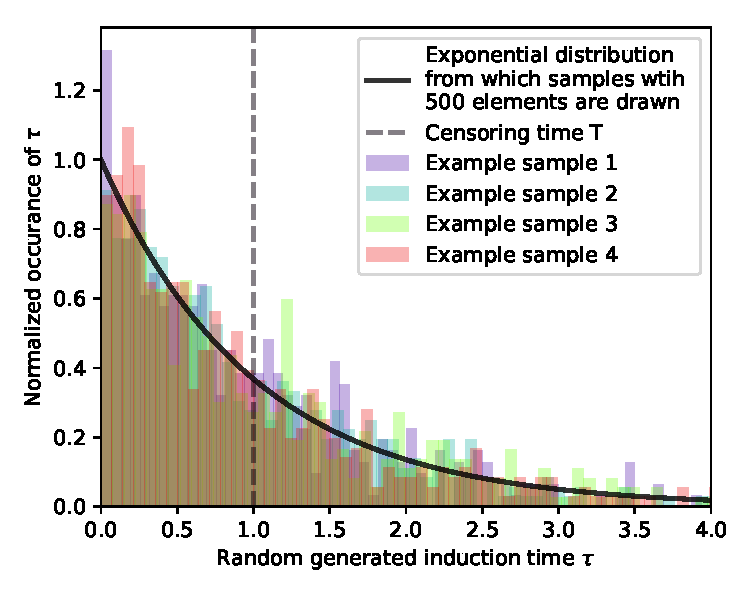
\includegraphics[width = 0.4 \textwidth]{mc_random_sample.pdf}} \hspace{0.5cm}
\subfloat[Distribution of $\hat{\kappa}$ for the previously generated MC samples. The distribution can be described mostly by mean and standard deviation as the number of estimates in the tails are small.]{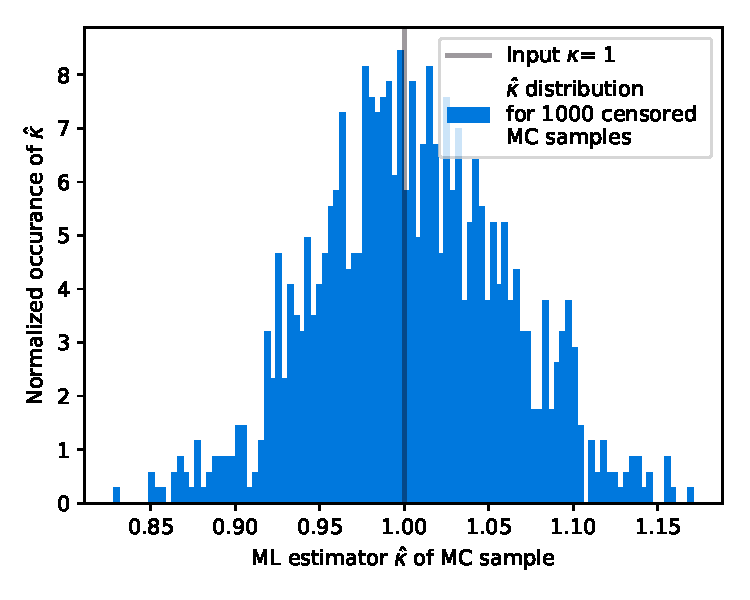
\includegraphics[width = 0.4 \textwidth]{k_estimator_distribution.pdf}}  
\caption[Monte Carlo uncertainty estimation example]{Exemplary samples for a given $\kappa$ as well as the distribution of estimates calculated from the random samples. The uncertainty on $\hat{\kappa}$ is approximated by the standard deviation of the distribution from the corresponding Monte Carlo analysis at a given $\kappa$.}
\label{fig:mc_example}
\end{center}
\end{figure}
Concerning the uncertainty in detail we can ask how long a simulation should be to yield precise results. For this we can first look at the case where $1 \gg \kappa T$ corresponding to a simulation where all boxes showed an nucleation event. In this case we have seen before that $\hat{kappa}^{-1} = \frac{1}{N} \sum_{i=1}^N t_i$. As we assume that the $t_i$ are exponentially distributed we further know that $\sigma_{t} = \kappa^{-1}$. The Gaussian error propagation then results in
\begin{align}
\label{eqn:uncertainty_k_gg}
\frac{\sigma_{\kappa}}{\kappa} = \frac{1}{\sqrt{N}} \; \text{.}
\end{align}

%\begin{align}
%\label{eqn:uncertainty_k_gg}
%\frac{\sigma_{\kappa}}{\kappa} &=\frac{1}{\kappa} \sqrt{\sum_{i=1}^N \left( \frac{\partial \kappa}%{\partial t_i} \right)^2 \sigma_{t_i}^2 }\\ 
%& \; \; \, \vrule
%  \begin{aligned}[t]
%  \raisebox{0.9cm}{ \makebox[1cm]{}} \text{with }  \frac{\partial \kappa}{\partial t_i} &= %\frac{\partial}{\partial t_i} \left( N \left( \sum_{i=1}^N t_i \right)^{-1} \right)\\
%  &= -N\left( \sum_{i=1}^N t_i \right)^{-2}  = \frac{\kappa^2}{N} \; \text{,} \\
% \raisebox{-0.4cm}{ \makebox[1cm]{}} \text{and } \sigma_{t} &= \kappa^{-1}
%  \end{aligned} \nonumber\\
% &= \frac{1}{\kappa} \sqrt{ N \left( \frac{\kappa^2}{N}\right)^{2} \kappa^{-2} } \\
% &= \frac{1}{\sqrt{N}}
%\end{align}
%\todo{Is das eine Tautologie!?}

Similarly we can take the limit of $1 \ll \kappa T$ which is the case when the mean nucleation time is much larger than the simulation time and therefore only a small fraction of the boxes hosted a nucleation event. In this case we can expand the estimator in the fraction of nucleated trajectories $\frac{n}{N}$ to find $\hat{\kappa} \approx \frac{n}{N} \frac{1}{T}$. In this case the decrease of nucleations events due to a smaller amount of available total volume is not seen yet, and the only information about the nucleation rate is obtained from the number of boxes with nucleations compared to the number of total amount of boxes used. As $n$ is Poisson distributed we know that $\sigma_n = \sqrt{n}$. Fixing N and T and using the expectation value of nucleations $n = N \kappa T$ the Gaussian error propagation for the relative uncertainty is given in \autoref{eqn:uncertainty_k_ll}.

\begin{align}
\label{eqn:uncertainty_k_ll}
\frac{\sigma_{\kappa}}{\kappa} &= \frac{1}{\kappa} \frac{\sqrt{n}}{NT} \nonumber\\
&=\frac{\sqrt{N \kappa T}}{N T \kappa} \nonumber\\
&=\frac{1}{\sqrt{N \kappa T}}
\end{align}

Finally we are also able to not only look at limits analytically, but also to approximate the relative uncertainty directly by means of the aforementioned Monte Carlo method. For this purpose the same procedure as before is used. The number of elements per sample is consistently with the performed simulations taken to be 500 and to archive good precision the standard deviation of 1000 samples is used for the uncertainty. As can be seen in \autoref{fig:relative_uncertainty} the fluctuations between different evaluations becomes rather small, but increase if using a lower number of samples. To compare the analytically derived limits of the uncertainty with the Monte Carlo results both are drawn into \autoref{fig:relative_uncertainty}.

\begin{figure}[ht]
\begin{center}
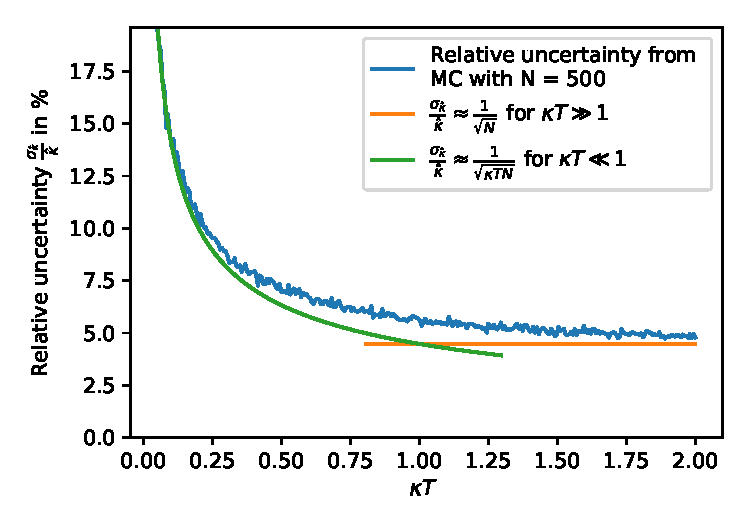
\includegraphics[width = 0.65 \textwidth]{rel_uncertainty_k.pdf}
\caption[Nucleation rate uncertainty depending on measurement time]{Relative uncertainty of the ML estimator for varying $\kappa T$. The x scale is chosen dimensionless such that it indicates the simulation time in comparison to the characteristic nucleation time.}
\label{fig:relative_uncertainty}
\end{center}
\end{figure}

We find that for the limits of $\kappa T \ll 1$ as well as $\kappa T \gg 1$ Monte Carlo results and analytical results are in good accordance while in between the analytical limits only can be used as a rough estimate.\\

What can be seen from \autoref{fig:relative_uncertainty} is that the uncertainty of the estimation drops sharply until about half of the characteristic time, after which it only gains little more precision. This is not surprising as the information is contained in the nucleation times and rather fast many nucleations have occurred and the long simulation times add only little of further nucleations. Thus simulating until all boxes had an nucleation event is only necessary if one want s to use the simpler arithmetic mean of the induction times as a characteristic time, or if any other constraints make it necessary to reach nucleation of all boxes.

\section{Nucleation rate comparison}
\label{sec:nucleation_rates}
Finally we are able to evaluate the induction time distribution to find the rates given in \autoref{fig:nucleation_comparison}.

\begin{figure}[h!]
\centering
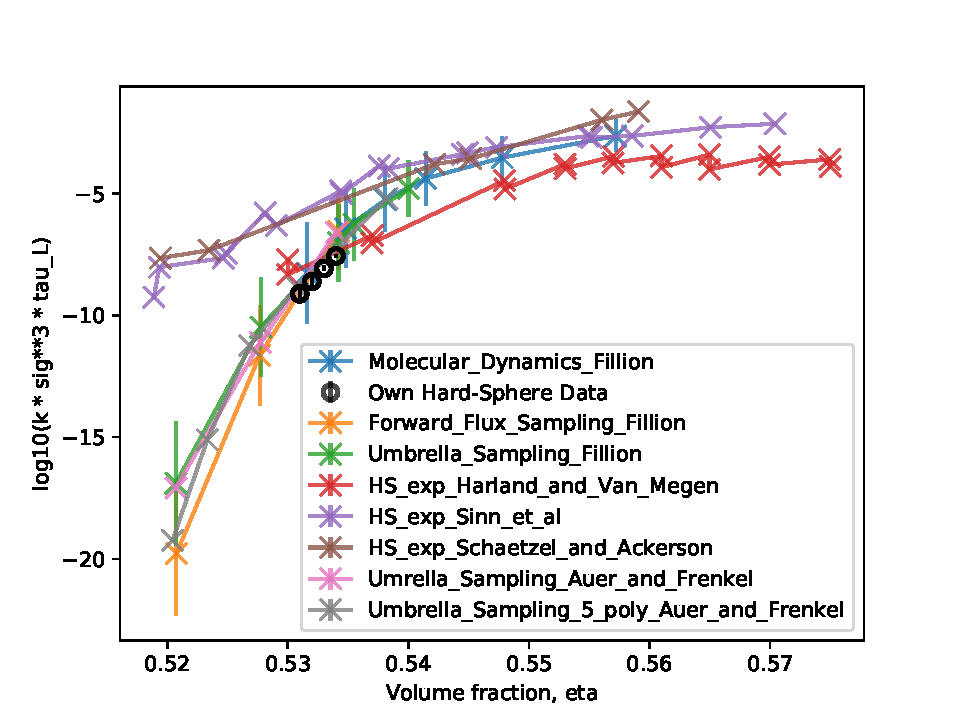
\includegraphics[width=0.7 \linewidth]{nucleation_rate_comparison.pdf}
\caption[Nucleation rate comparison with literature values]{Some examples of nucleation times in the hard sphere system for varying volume fractions from the literature have been collected, to compare with the own measured data points. All data points have for this purpose been scaled by the self-diffusion constant to make comparisons between different experiments possible, as the diffusion sets the timescale at which the system evolves.}
\label{fig:nucleation_comparison}
\end{figure}

From the diagram we can state that our Event driven molecular dynamics simulations confirm the previous simulation results that stood against the experimentally found ones. Further these results are calculated together with their statistical uncertainty, which is mostly visible for the data point at $\eta = 53.1 \%$ but is indicated for the others as well but due to the logarithmic scaling almost not visible.

All Nucleation rates that can be found.-> may hap ask Hajo.\\
-nucleation rates without\\
-nucleation rates with small particles\\


\section{Memory kernels of nucleating ensemble}
\label{sec:memory_kernels}

Following the approach of Hugues Meyer to calculate memory kernels for an ensemble of trajectories\cite{Meyer2019a}, memory kernels for trajectories of about one million particles at volume fractions between $\eta = 53.1\% - 53.4\%$ as well as for a system containing 16384 particles and a volume fraction of $\eta = 54.0\% $ have been calculated. While the first ensemble was not simulated up to the point where almost all boxes where nucleated, and the transition width can be assumed to be large as it takes long simulations for clusters to fill up the large box, the second is chosen to fulfill both objections with parameter given in \autoref{tab:system_16k_mem}.\\

\begin{table}[ht]
\centering
\begin{tabular}{c|c}
Parameter & Value \\ \hline
N & 16384 \\
eq\_steps/particle & 5000 \\
pr\_steps/particle & 200000 \\
$\eta_i$ & 45.0 \% \\
$\eta_f$ & 53.4 \% \\
\end{tabular}
\caption[Simulation parameters of data production system with 16384 particles]{Input parameters of simulations on the NEMO HPC cluster. The large number of production steps is chosen together with the final volume fraction $\eta_f$ in a way to simulate nucleation and full crystalization of the boxs in almost all cases as can be seen in the top diagram of \autoref{fig:cluster_growth_example}. Furthermore the small box size leads to a small transition width $\Delta$ of about $150 \delta t$ corresponding closley to the width of the memory kernel.\cite{Meyer2021}} 
\label{tab:system_16k_mem}
\end{table}



Still the memory kernel of the large system has been calculated but except of the Markovian contribution only a slight idea of the memory kernel was visibible, indicating that the sample is not sufficently long or that the largest cluster is not an appropriate observable for nucleation in large systems.\\



To compare the memory kernel with direct measurements of the observable the evolution of the ensemble is depicted in the top of \autoref{fig:cluster_growth_example}. The trajectories have been normalized by the number of particles in the box and some statistical properties likes percentiles and arithmetic mean are also shown as the large number of trajectories otherwise makes it hard to distinguish the actual density of lines at some points. At the bottom of the figure the share of trajectories at different stages of the nucleation process is identfied. For this it is assumed that trajectories below an normalized largest cluster of 0.1 can be identified as not nucleated, normlaized trajectories above 0.5 as fully crystallized and all trajectories in between as in the process of filling the box.\\
As there is no clear analysis yet on how the direct quantities and the memory kernel are related, the differentiation tries to relate intuitively corresponding quantities of the memory kernel and the direct observable.\\

\begin{figure}[ht]
\centering
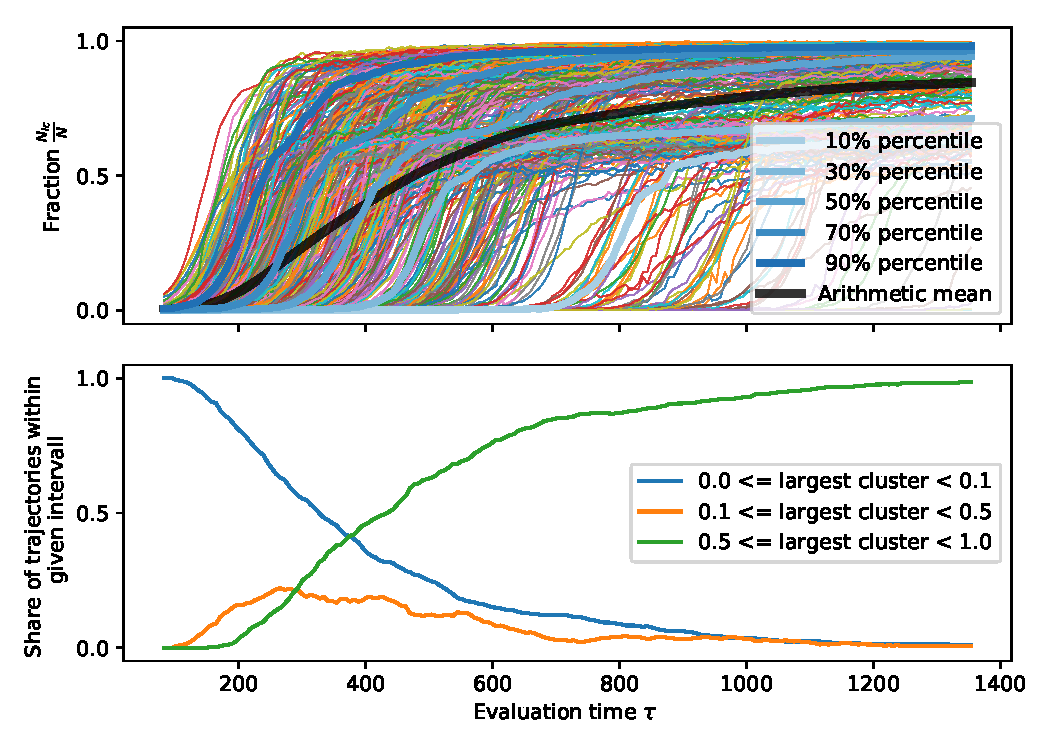
\includegraphics[width=0.7 \linewidth]{cluster_growth_quantities.pdf}
\caption[Largest cluster trajectories of small system with percentiles and average]{Top: Normalized trajectories of largest cluster with percentiles and arithmetic mean indicated. It can be observed that some fraction of the trajectories nucleates in more than one step where at first only about 60\% of the box is filled by the crystal and at later times they sometimes crystalize further until almost the complete box is filled by the solid phase. From \autoref{eqn:solid_fraction_result} we would expect a solid fraction of 80\% by volume corresponding closely to the expected solid fraction by particles.\\
Bottom: Fraction of trajectories within intervals chosen to identify nucleated trajectories, momentary growing trajectories and fully nucleated trajectories. As the growth process is much faster than the distribution of nucleations, the orange curve roughly resembles the derivative of the other two curves.}
\label{fig:cluster_growth_example}
\end{figure}


%The memory kernel of the second ensemble of trajectories is shown in \autoref{tab:system_16k_mem}. 


While for the large system only little of the crystallites reached the box boundaries in this latter almost all clusters fill the whole box at the ende of the simulation. As pointed out earlier this finite phase transition time is of the same size as the width of the memory kernel at the mean induction time of the trajectories. As we can see in \autoref{fig:memory_kernel} the shape of a memory kernel slice at some reference time is rather simple. For this reason we use a Gaussian fit to approximate the width and amplitude of the kernel. For this purpose we neglect the Markovian part of the kernel at around $t_1-t_2 \approx 0$. To validate the fit results we further use the FWHM, where the maximum is determined by the mean value of the peaks crest.\\
As the properly normalized result for both methods are in good agreement, we can conclude that the shape of the memory kernel in this case is rather easily defined by a width and an amplitude over time which is depicted in \autoref{fig:memory_kernel}.


\begin{figure}[ht]
\begin{center}
\subfloat[Slice through memory kernel at the given reference time. With the data the excluded Markovian part of the kernel is depicted. Further the full width at half maximum (FWHM) is shown as a first measure of the kernel width as well as a Gaussian fit. The FWHM is normalized to the value of a corresponding Gaussian curve.]{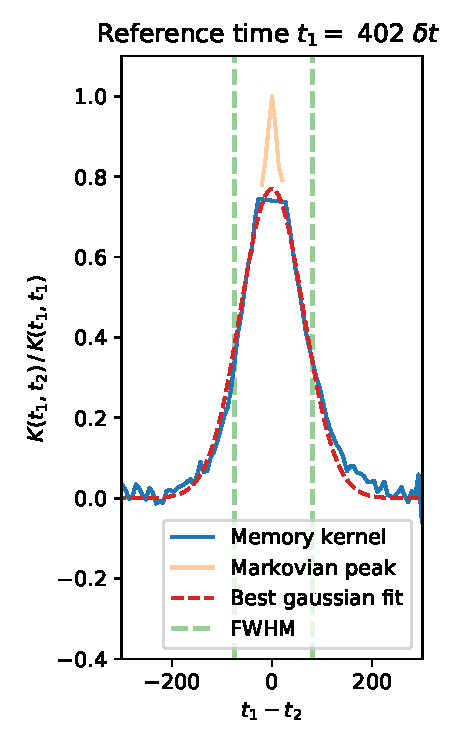
\includegraphics[width=0.37 \linewidth]{example_memory_kernel.pdf}} \hspace{0.5cm}
\subfloat[Top: Width of the memory kernel slices by FWHM and Gaussian fit. The FWHM is normalized to the value of a corresponding Gaussian curve.
Bottom: Amplitude of the memory kernel slice by on the one hand using the mean value of the data around the maximum and on the other by using the amplitude derived from the best Gaussian fit. The amplitude derived from the maximum value is normalized to the value of a corresponding Gaussian curve.]{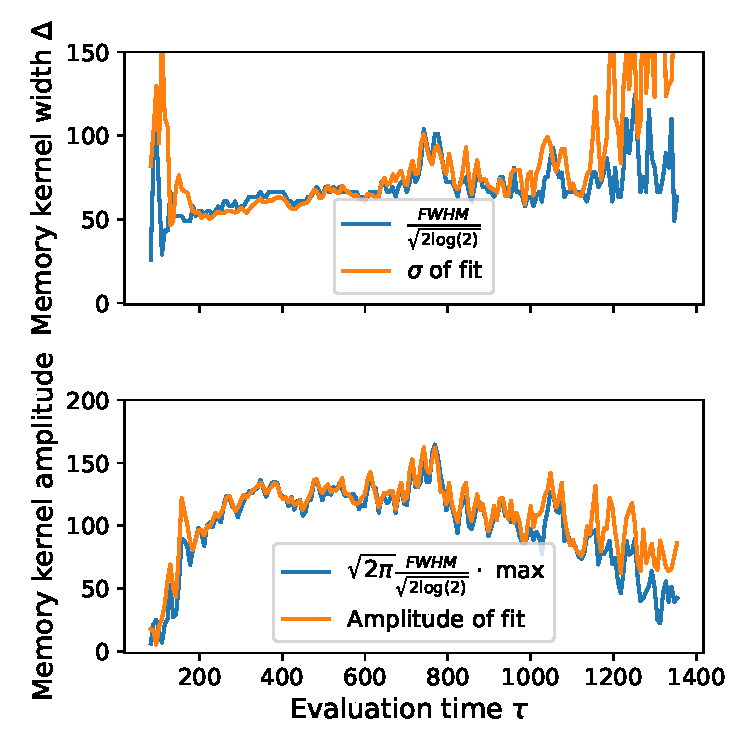
\includegraphics[width=0.59 \linewidth]{memory_kernel_shape.pdf}}
\caption[Width and amplitude of memory kernel with example slice]{Example memory kernel together with width and amplitude depending on time.}
\label{fig:memory_kernel}
\end{center}
\end{figure}

As we see the width of the memory kernel sections is more or less constant over the whole measurement with the exception that it becomes very noise at the end.\\
The amplitude in comparison increases at the beginning, remains over a prolonged period of time constant and then declines towards the end of the measurement.\\
As pointed out in our article\cite{Meyer2021} the width of the memory kernel seems to depend on the transition width. As the width in this case is mostly given by the arbitrarily chosen box size it might be possible that we only can see this effect, and otherwise present memory effects are buried beneath. To find these possibly covered memory effects one could generate trajectories with a purely Markovian approach like Brownian dynamics, that corresponds closely to the characteristic properties found for the hard sphere system. Calculating memory kernels from these purely Markovian ensembles would make it possible to compare with the a priori non Markovian ensembles, possibly giving more insight.\\
An other approach would be to use the committer probability of the largest cluster as an observable, as it would not include a direct system size dependence, that possibly buries other memory effects.
